\section{Problem statement} \label{sec:problems}
\subsection{Road Congestions}
After Munich, Berlin is the city with the most traffic jams in Germany. Peak hour traffic jams are mostly caused by the commuting people. According to TomTom \cite{tomtom} data, commuting people need to add 12 minutes per 30 min. in the morning and 16 min. per 30 min. in the evening. As a normal employee works around 48 weeks per year and 5 days per week this results in an average time lost of 48 hours in the morning and 64 hours in the evening per 30 minutes additional traveling time per year. At Figure \ref{averageCongestion} the average percentages of the weekly congestion per hour are visible.

%nogal gigantische figuur, kversta datie groot genoeg moet afgebeeld worden, dus mss in appendix? of toch iets kleiner maken?
\begin{figure}[h!]
	\centering
	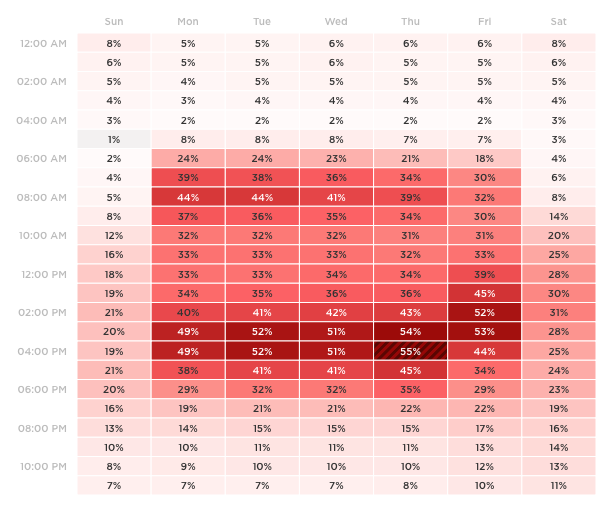
\includegraphics[width=0.55\textheight]{ProblemsFigures/TOMTOMWeeklyAverageCongestion}
	\caption{The average percentage of weekly congestion per hour in Berlin }
	\label{averageCongestion}
\end{figure}

% 'expo real': drukletters? Hoofdletter? 
\subsection{Train Delay}
A second big problem for commuting people is train delay. Typically the commuters use  the S-Bahn train (\ref{sebsec:sBahn}) to enter the city and the fast ICE train if they live at a greater distance of Berlin. As Jens-Peter Schulz, CEO of Dresdner Real Estate Investment Holding \& Chairman told in an article for expo real: 'Germany travelers cheer if their train arrives less than 10 minutes late'. Because the majority of the commuting people live near Berlin we will only analyze the S-Bahn train. People mostly complain that the complete railway system in Germany is not very flexible, once a train has a delay it just causes a lot of other delays. Especially when the train becomes very crowded, the stop time of the trains increases every time. As that train arrives in a transfer station with a delay, the other trains wait on that train so it's possible for the passengers to transfer, which results in more trains with a delay. 

\subsection{Ticket price} \label{subsec:ticketprice}
The ticket prices for public transport in Berlin are the 5th most expensive of the whole world (Figure \ref{pricePT}). As a single ticket costs around \texteuro{3.16} and the majority of the commuting people need to cover on average 14.3 Km (Figure \ref{averageComDis}) to go working. With an average fuel consumption of 4.1 L/100Km (2020) and a fuel price of  \texteuro{1,65}/L (2021), this means going to work with the car costs around \texteuro{1} --car parks payment not included. So for people that own a car and do have a car parks spot near their work, it financially seems to be more attractive to take the car. 

\begin{figure}[h!]
	\centering
	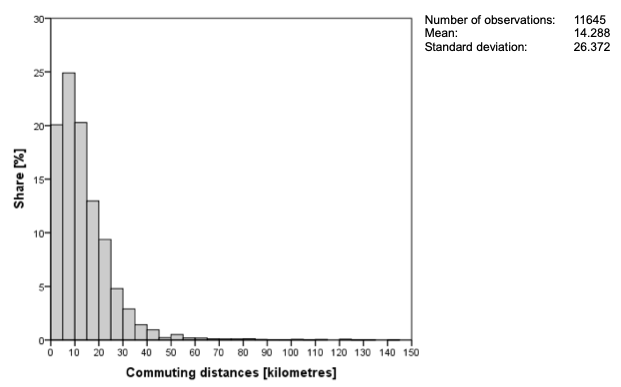
\includegraphics[width=0.55\textheight]{ProblemsFigures/averageCommutingDistance}
	\caption{The average distance the commuting people cover in 2012. }
	\label{averageComDis}
\end{figure}

\section{Proposals}
In this section some proposals are given to solve the problems discussed in section \ref{sec:problems}. There is not one right solution for these problems, but as one problem is solved this will also have an impact on the others. When trains are more reliable and cheaper, more people will use them instead of taking their car, which resolves in less road congestions. The other way around is possible as well when there are less road congestions, more people will take the car resolving in smaller delays for the trains as they will not be overcrowded. The subsections \cref{subsec:RoadTax,subsec:parkin,subsec:resSys,subsec:ticketPriceSolution} will propose an individual solutions for each problem.

\subsection{Road Pricing} \label{subsec:RoadTax}
One of the answers the the congested roads problem could be a road pricing. There are two possibilities of road pricing: either distinct prices on different roads to spread the traffic better or a dynamic road pricing that would change in function of the hours. Both can obviously be combined as well. \\ \newline
Having distinct prices on different roads is an easy way to shift traffic from one place to an other. The investment to make this possible is also relatively low. Although there's in Germany no road pricing for cars at the moment, this does not mean that it is necessary to develop a whole new system. It is possible to add just one road segment where a fee needs to be paid. Think of a tunnel, bridge or even just a road, the only investment to make is a place to stop and pay (most of the time using a barrier). Most people will automatically avoid this road and take an other one. When a congestion occurs because of an incident, the decision to make that road segment free can be made. As a result of this decision the congestion on the other road will solve much easier. The downside of this solution is when the road isn't free, it will be used much less than before and therefore the other roads will be more busy. A popular example of this solution is situated in Antwerp where the ring is very often congested. There is an other road to pass Antwerp, which has the Liefkenshoektunnel on its path. In this tunnel normally you need to pay a fee for passing. When there is a major incident on the normal ring, this tunnel is made free resulting in a smaller traffic jam.     \\ \newline
Making a variable road pricing system will spread the traffic more even through the day. Such a system means that when driving in the peak hours the price of the road is greater then when driving on more calm moments. People that do not necessary need to travel/commute at peak hours will wait or leave earlier to avoid the more expensive road pricing. It is inconvenient that a new system needs to be introduced in Germany (or at least in Brandenburg and Berlin), considering the time and work it will need to prepare, draw up and integrate. \\ \newline
These systems already exist in other countries, but are most of the time used for trucks: a receiver inside the vehicle recognizes the different pricing zones. Some examples are ViaPass in Belgium and ViaToll in Poland. The variable road pricing can be fixed (always the same every day) or dynamic (changing on the current situation). On Figure \ref{fig:dynroad} (\cite{dynRoadPrice}) it's visible that the average delay decreases a lot in the peak hours.

\begin{figure}[h!]
	\centering
	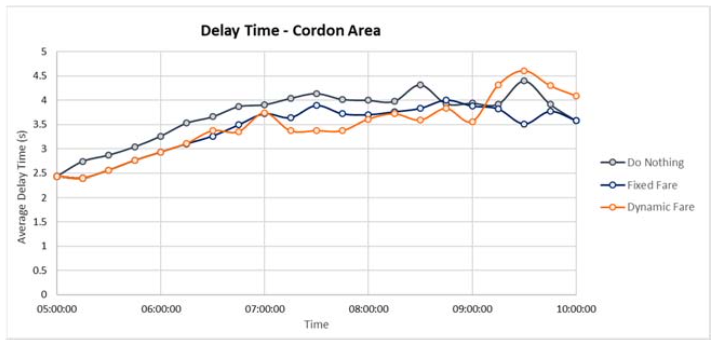
\includegraphics[width=0.55\textheight]{ProblemsFigures/dynamicRoadPricing}
	\caption{A graph that compares the average delay between different road pricing systems. }
	\label{fig:dynroad}
\end{figure}

\subsection{car parks in urban fringe} \label{subsec:parkin}
An other answer for the many traffic jams could be the so called park and ride car parks with easy accessible roads. At the moment there are a few of those in the urban fringe but you still need to pay a small amount to park there. This can only be a good solution for the road congesting problem if there is a good connection from that car park to the city centre. Some ideas are building the car parks near a U-Bahn of S-Bahn train stop, adding a bus stop at the car parks or making a bike sharing rental on the site. \\ \newline 

%de deelzinnen en zinnen staan lik allemaal los van elkaar?
The build of these car parks and additional accommodations are big investments for the city, the roads to these car parks need to be big enough to handle the peak hours. This could also mean the start of making the city centre car free as that is something happening in a lot of big cities at the moment. An example of this is the Flanders expo car parks in Ghent where you can take the tram to the city centre. 

\subsection{Variable train ticket pricing} \label{subsec:ticketPriceSolution}
A way to address the train delay problem is a dynamic train ticket price system. It would work a bit like the variable road pricing for the cars. This system would work with a magnetic card on which you put some money to pay the train ride (this can be enlarged to the whole public transport system). There would be fixed prices for each trip as it is now, except the only difference would be that the prices are divergent for different hours. This would spread the travelers more over the whole day. \\ \newline
 Now, a lot of people take the train to go to Berlin whenever they want. At the hand of this system they would first of all think when they want to take the train, so it's as cheap as possible. As we addressed in \ref{subsec:ticketprice}, the ticket price for the public system is very high comparing to other ways of commuting, therefore the prices in the peak hours shouldn't increase, but the ticket price in the non-peak hours should decrease. An additional feature to this system would be diverse subscriptions for the different times: a subscription for peak hours would be more expensive than one for non-peak hours and would be usable during non-peak hours, but not the other way around. 
 
\subsection{Train reservation system}\label{subsec:resSys}
A second solution for the train delay problem would be a train reservation system. By introducing this, the train providers can anticipate on unexpected large amounts of travelers by adding some wagons to the trains. As it's obviously not possible to make a reservation on a train mandatory, there needs to be an other way to make reservations more attractive. \\ \newline
This could be done by charging lower prices when you reserve a ticket (whether or not at least 24 hours before departure). A second way would be to guarantee a place to sit on each train, although this would be much more difficult to succeed as the rule on a train is most of the time first come first take. 

%kversta de zin niet
The system would be connected to the magnetic card, so when you pay the amount is less then it would be when you didn't reserve a spot. The system of reserving a place on a train is already used on the high speed trains as the Thalys and the TGV.  

\subsection{Political change}\label{politicalChange}
Ultimately, the politics in Germany cannot be forgotten. As it is improving at the moment, the relation politics-public transport isn't as coherent as in the other countries. The car industry in Germany is one of the biggest industries of the whole country, consequently this industry has a big influence on the German economy and politics. The car commerce is in the eyes of the politicians more beneficial to the country, resulting in a higher priority in the past and present. That's the reason why a lot of the train infrastructures are old and are being replaced at this moment. \\ \newline 
The last few years it's clear that the positive environmental impact of the public transport is very important, so much more money is invested in the public transport by the government. These new investments are on long term a good improvement against the train delays, but at short term they cause a lot of extra delays. On Figure \ref{fig:typesOfTransport} it's clear that there is still a lot of improvement possible according to more public transport and rail use compared with the car use. 

\begin{figure}[h!]
	\centering
	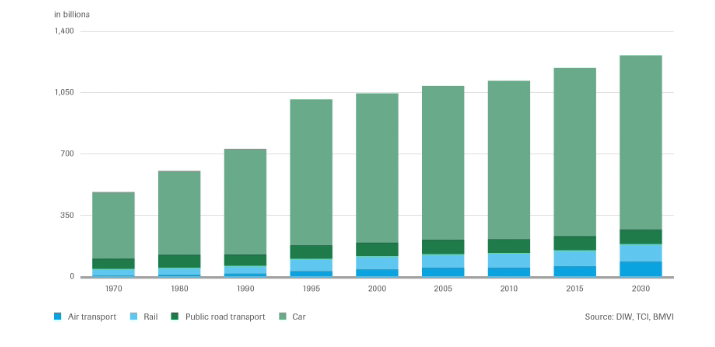
\includegraphics[width=0.55\textheight]{ProblemsFigures/typesOfTransportGermany}
	\caption{The evolution in the different used types op transport.}
	\label{fig:typesOfTransport}
	
\end{figure}

